\documentclass{article}

\usepackage[left=2cm,right=2cm,top=2cm,bottom=2cm]{geometry} 

\usepackage[utf8]{inputenc}   % otra alternativa para los caracteres acentuados y la "ñ"
\usepackage[           spanish % para poder usar el español
                      ,es-tabla % para los captions de las tablas
                       ]{babel}   
\decimalpoint %para usar el punto decimal en vez de coma para los números con decimales

%\usepackage{beton}
%\usepackage[T1]{fontenc}

\usepackage{parskip}
\usepackage{xcolor}

\usepackage{caption}

\usepackage{fancyvrb}

\usepackage{enumerate} % paquete para poder personalizar fácilmente la apariencia de las listas enumerativas

\usepackage{graphicx} % figuras
\usepackage{subfigure} % subfiguras

\usepackage{amsfonts}
\usepackage{amsmath}

\usepackage[formats]{listings}
\lstdefineformat{R}{~=\( \sim \)}
\lstset{basicstyle=\ttfamily,format=R}

\definecolor{gris}{RGB}{220,220,220}
	
\usepackage{float} % para controlar la situación de los entornos flotantes

\restylefloat{figure}
\restylefloat{table} 
\setlength{\parindent}{0mm}


\usepackage[bookmarks=true,
            bookmarksnumbered=false, % true means bookmarks in 
                                     % left window are numbered
            bookmarksopen=false,     % true means only level 1
                                     % are displayed.
            colorlinks=true,
            allcolors=blue,
            urlcolor=blue]{hyperref}
\definecolor{webblue}{rgb}{0, 0, 0.5}  % less intense blue


\title{\Huge SWAP: Preparación de las herramientas\vspace{10mm}}

\author{\huge David Cabezas Berrido \vspace{10mm} \\ 
  \huge dxabezas@correo.ugr.es \vspace{10mm}}

\begin{document}
\maketitle
\tableofcontents
\newpage

\section{Objetivos}

El objetivo de esta primera práctica es la puesta en marcha de dos máquinas virtuales idénticas que puedan conectarse a internet y entre sí.
Así como la instalación y configuración de ciertos servicios y herramientas como son Apache, PHP, MySQL, SSH o CURL.

\section{Creación de las máquinas e instalación del sistema}

Comenzamos creando dos máquinas virtuales idénticas, seleccionamos Ubuntu-64b y la configuración recomendada (1 core, 1GB de RAM y 10GB de disco dinámicos).

Ambas máquinas vienen con un adaptador de red NAT por defecto, añadimos un segundo adaptador de red Host-only (\texttt{Settings -> \ Network 
	-> \ Adapter 2 -> \ Host-only Adapter})
para que las máquinas puedan comunicarse entre sí. Si no tenemos ninguno, lo podemos crear en \texttt{File -> \ Host Network Manager -> \ Create}.

\begin{figure}[H]
	\centering
	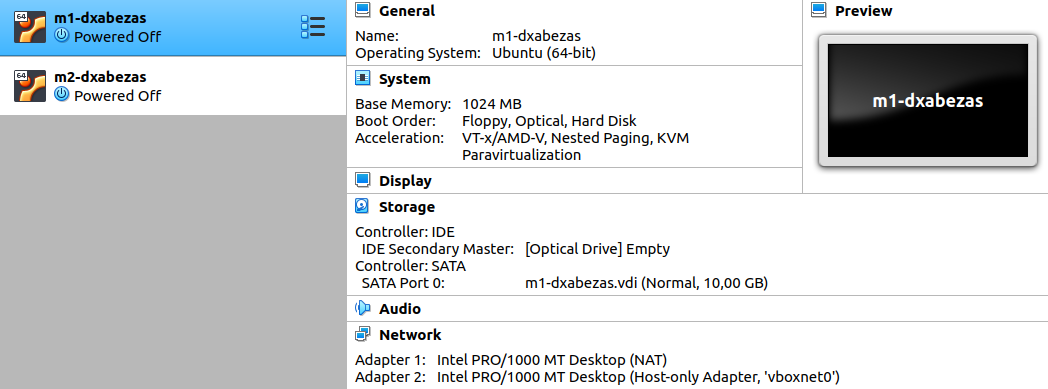
\includegraphics[width=160mm]{imgs/maquinas}
	\caption{Resumen de la configuración de la máquina M1. Observamos que tiene los dos adaptadores de red que hemos comentado.}
	\label{fig:maquinas}
\end{figure}

Seguidamente, instalamos Ubuntu Server 18.04 LTS en ambas máquinas. Podemos descargar la ISO de la página oficial. Creamos en las dos máquinas perfiles idénticos, con usuario \textbf{dxabezas} y constraseña \textbf{Swap1234}.

\begin{figure}[H]
	\centering
	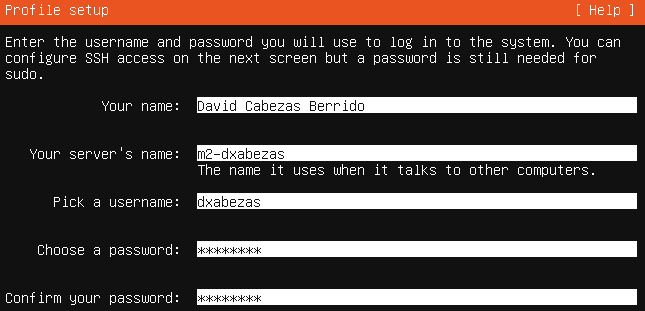
\includegraphics[width=160mm]{imgs/perfil}
	\caption{Creando el perfil en la máquina M2.}
	\label{fig:perfil}
\end{figure}

Durante la instalación escogemos siempre las opciones recomendadas, con la excepción de instalar OpenSSH.

\section{SSH}

Ya tenemos OpenSSH instalado en ambas máquinas. Si durante la instalación no lo hubiésemos marcado, tendríamos que ejecutar:

\begin{verbatim}
	sudo apt-get install openssh-client
	sudo apt-get install openssh-server
\end{verbatim}

Con \texttt{ifconfig}, podemos ver la dirección IP de cada máquina:

\begin{figure}[H]
	\centering
	\subfigure[Máquina 1.]{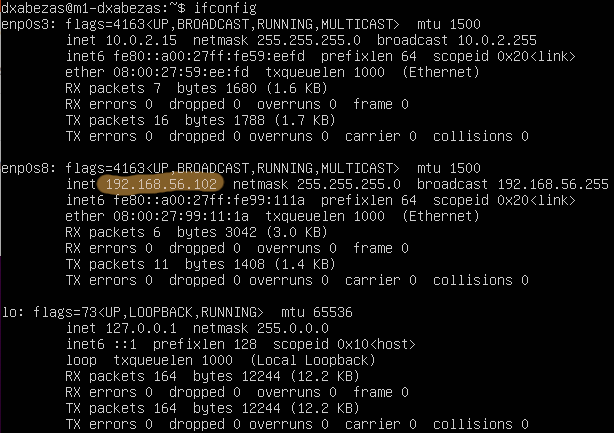
\includegraphics[width=87mm]{imgs/ifconfig1}}
	\subfigure[Máquina 2.]{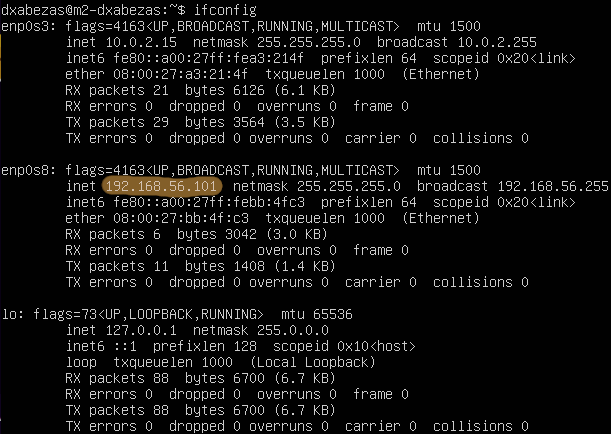
\includegraphics[width=86.5mm]{imgs/ifconfig2}}
	\caption{Direcciones IP de ambas máquinas.}
	\label{fig:ifconfig}
\end{figure}

Nos conectamos de una máquina a otra, ejecutando \texttt{ssh user@ip}.
\begin{figure}[H]
\centering
\subfigure[M1 se conecta a M2.]{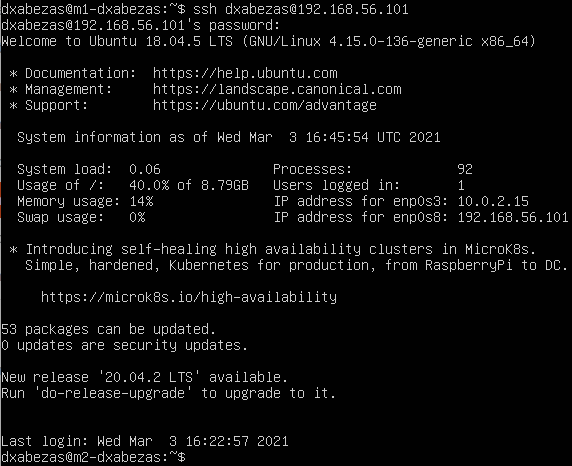
\includegraphics[width=86mm]{imgs/ssh1}}
\subfigure[M2 se conecta a M1.]{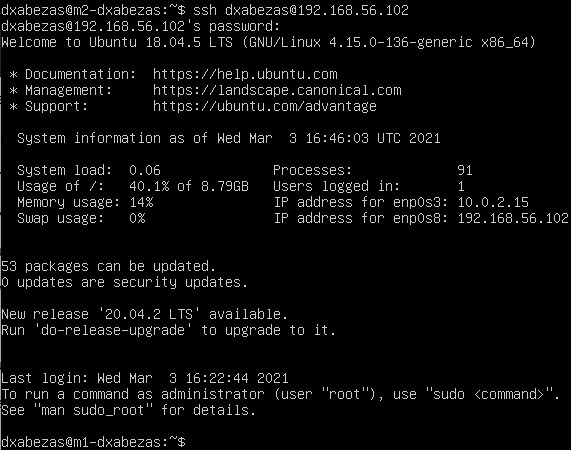
\includegraphics[width=88mm]{imgs/ssh2}}
\caption{Cada máquina se conecta a la otra por SSH con el usuario que creamos (dxabezas, Swap1234).}
\label{fig:ssh}
\end{figure}

\textbf{NOTA:} En lo que viene a continuación, la dirección IP de M1 es la que termina en 1 y la de M2 es la que termina en 2.
En la siguiente sección
explico cómo las intercambio.

Ahora vamos a configurar SSH, para ello modificamos el fichero \texttt{/etc/ssh/sshd\_config}, donde se encuentra la configuración
del servicio \texttt{ssh-server}. \texttt{/etc/ssh/ssh\_config} es para la configuración de \texttt{ssh-client}.
Por ejemplo, podemos modificar el puerto del 22 (por defecto) al 2222 con la línea \texttt{Port 2222}. Para hacer efectivos los cambios,
guardamos el archivo y reestauramos el servicio con

\begin{verbatim}
	sudo service ssh restart
\end{verbatim}

Ahora desde la otra máquina
nos conectamos, pero debemos indicar el puerto explícitamente (con la opción \texttt{-p}) al no tratarse del por defecto.

\begin{figure}[H]
	\centering
	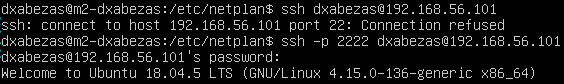
\includegraphics[width=140mm]{imgs/ssh-port}
	\caption{La máquina 2 se intenta conectar a la máquina 1. El primer intento fracasa porque intenta conectarse al puerto por defecto.}
	\label{fig:ssh-port}
\end{figure}

Una buena práctica desde el punto de vista de la seguridad es deshabilitar el root login (\texttt{PermitRootLogin no}). De esta manera,
nadie se puede conectar como root por SSH, tendrá que obtener permisos de superusuario una vez logueado en el sistema mediante sudo.

Finalmente, configuraremos el acceso sin contraseña mediante clave pública. Desde la máquina M2 generamos un par de claves con
\texttt{ssh-keygen -t rsa}, nos da la opción de poner una passphrase por si tememos que alguien pueda acceder a nuestro dispositivo.

\begin{figure}[H]
	\centering
	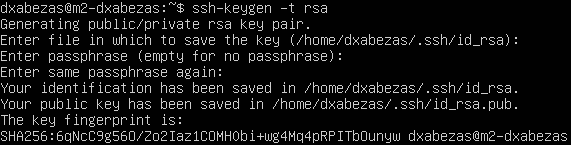
\includegraphics[width=140mm]{imgs/keygen}
	\caption{La máquina 2 genera un par de claves (pública y privada).}
	\label{fig:keygen}
\end{figure}

Ahora copiamos la clave pública en M1 ejecutando (desde M2)
\begin{verbatim}
	ssh-copy-id -p 2222 dxabezas@192.168.56.101
\end{verbatim}

nos pide la contraseña (Swap1234) y nos dice que se ha añadido 1 clave. Ahora nos podemos conectar con SSH sin poner sin que nos pida
la contraseña, nos pedirá la passphrase en caso de haber puesto una.

Hemos elegido crear la pareja de claves en los archivos por defecto (\texttt{$\mathtt{\sim}$/.ssh/id\_rsa} y
 \texttt{$\mathtt{\sim}$/.ssh/id\_rsa.pub}). De haber
seleccionado otros archivos, tendríamos que indicar con la opción \texttt{-i} el archivo de clave a copiar (pública) y a utilizar
para autenticarse (privada).

\section{Configuración de red}

Ya tenemos los dos adaptadores de red (NAT y Host-only) creados. Cuando instalamos el sistema se configuran por defecto,
pero podemos usar Netplan para realizar los cambios que deseemos.

Para ello, modificamos el fichero \texttt{00-installer-config.yaml} en la carpeta \texttt{/etc/netplan}, donde ya encontramos
 la configuración por defecto del adaptador NAT (interfaz \texttt{enp0s3}) y del adaptador Host-only (interfaz \texttt{enp0s8}),
 que reciben direcciones IP via DHCP. Podemos consultar las direcciones asignadas con \texttt{ifconfig} (Figura \ref{fig:ifconfig}).

\begin{Verbatim}[tabsize=4]
network:
	version: 2
	ethernets:
		enp0s3:
			dhcp4: true
		enpos08:
			dhcp4: true
\end{Verbatim}

En la Figura \ref{fig:ifconfig} también observamos que las direcciones obtenidas están ``cambiadas'', la máquina 1 recibió
 \texttt{192.168.56.102} y la máquina 2 la \texttt{192.168.56.101}. Esto se debe a que realizamos primero la instalación de la M2,
 pero ahora podemos cambiarlas manualmente para tener direcciones más intuitivas. También en la Figura \ref{fig:ifconfig} observamos
 que se utiliza la máscara de red \texttt{255.255.255.0} (24 bits a 1 y 8 bits a 0), la mantenemos añadiendo \texttt{/24} tras la dirección.
  Editamos el archivo con 
 \texttt{sudo nano 00-installer-config.yaml}. En la máquina 1 escribimos:

\begin{Verbatim}[tabsize=4]
network:
	version: 2
	ethernets:
		enp0s3:
			dhcp4: true
		enpos08:
			dhcp4: no
			addresses: [192.168.56.101/24]
			gateway4: 192.168.56.1
\end{Verbatim}

y en la M2 cambiamos a \texttt{192.168.56.102/24}. Para aplicar los cambios ejecutamos \texttt{sudo netplan apply}, podemos comprobarlos
con ifconfig y conectarnos por ssh desde la máquina anfitriona o la otra máquina para comprobar que funciona. Si ya nos conectamos
desde la máquina anfitriona antes de este cambio, habrá que borrar la fingerprint de known hosts primero.

\begin{figure}[H]
	\centering
	\subfigure[La IP de M1 ha cambiado.]{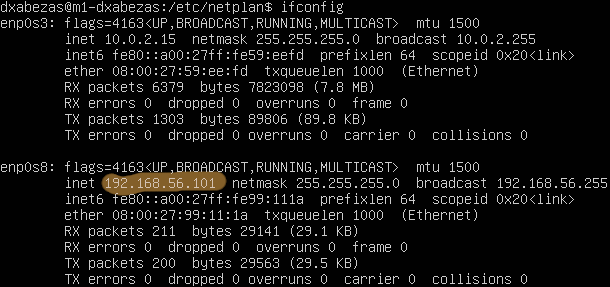
\includegraphics[width=88mm]{imgs/m1-ifconfig-static}}
	\subfigure[Nos conectamos a M1 desde el anfitrión con la nueva IP.]{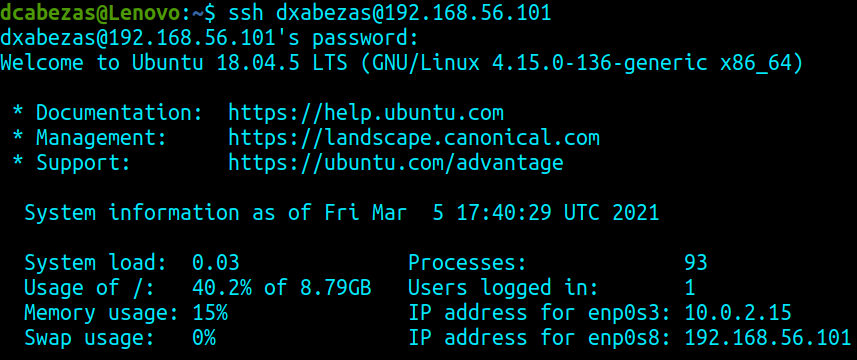
\includegraphics[width=84mm]{imgs/ssh-host}}
	\caption{Conexión por SSH desde el anfitrión a M1 con la nueva IP.}
	\label{fig:static-ip}
\end{figure}

\section{Servicios LAMP}

\subsection{Apache2}

Puesto que no marcamos los servicios LAMP durante la instalación, debemos instalarlos manualmente. Empezamos con Apache2,
en ambas máquinas ejecutamos:
\begin{verbatim}
	sudo apt install -y apache2
\end{verbatim}

Para comprobar la versión que hemos instalado usamos \texttt{apache2 -v}, y para comprobar que esté en ejecución, 
\begin{verbatim}
	sudo service apache2 status
\end{verbatim}

\begin{figure}[H]
	\centering
	\subfigure[Máquina 1.]{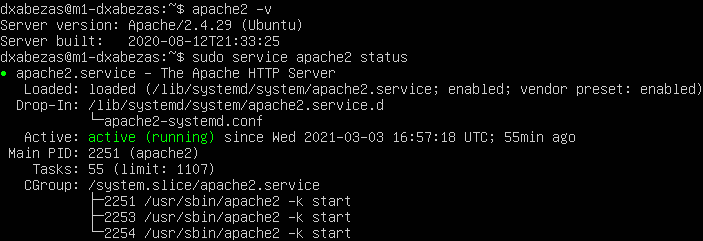
\includegraphics[width=120mm]{imgs/apache1}}
	\subfigure[Máquina 2.]{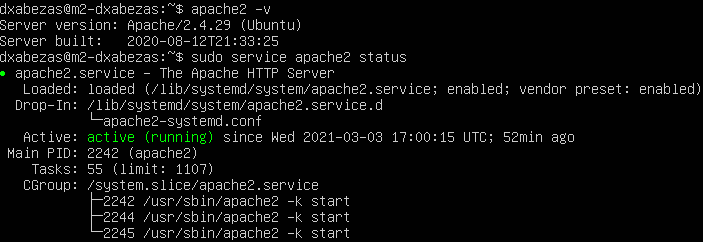
\includegraphics[width=120mm]{imgs/apache2}}
	\caption{Comprobamos la versión de Apache2 y que esté activo.}
	\label{fig:apache2}
\end{figure}

En la máquina 1 cambiamos el puerto de escucha al 8000 escribiendo \texttt{Listen 8000} en el fichero \texttt{/etc/apache2/ports.conf}.
En el fichero avisa de que modifiquemos también \texttt{/etc/apache2/sites-enabled/000-default.conf}, donde cambiamos la línea
\begin{verbatim}
	<VirtualHost *:80>
\end{verbatim}
por \texttt{<VirtualHost *:8000>}.

Ejecutamos \texttt{sudo apache2ctl configtest} para comprobar que está todo bien. Nos da un warning diciendo que le pongamos un
nombre de dominio al servidor, ya que actualmente se está usando (\texttt{127.0.1.1}). Lo cambiamos añadiendo la línea
\begin{verbatim}
	ServerName 192.168.56.101
\end{verbatim}
al fichero \texttt{/etc/apache2/apache2.conf}. También cambiamos el nombre a
\texttt{192.168.56.102} en la M2. Ahora la comprobación sólo nos devuelve Syntax OK.
 Reestablecemos el servicio para que se apliquen los cambios.

\begin{verbatim}
	sudo systemctl restart apache2
\end{verbatim}

Desde la máquina anfitriona podemos visitar las direcciones \texttt{192.168.56.101:8000} (M1, hemos cambiado el puerto de escucha)
 y \texttt{192.168.56.102} (M2, puerto 80 por defecto). Comprobamos que Apache funciona correctamente, nos sirve el fichero
 \texttt{/var/www/html/index.html}. Se puede cambiar el directorio modificando \texttt{DocumentRoot} en 
 \texttt{/etc/sites-available/000-default.conf}.
 
\begin{figure}[H]
	\centering
	\subfigure[M1, al puerto 8000.]{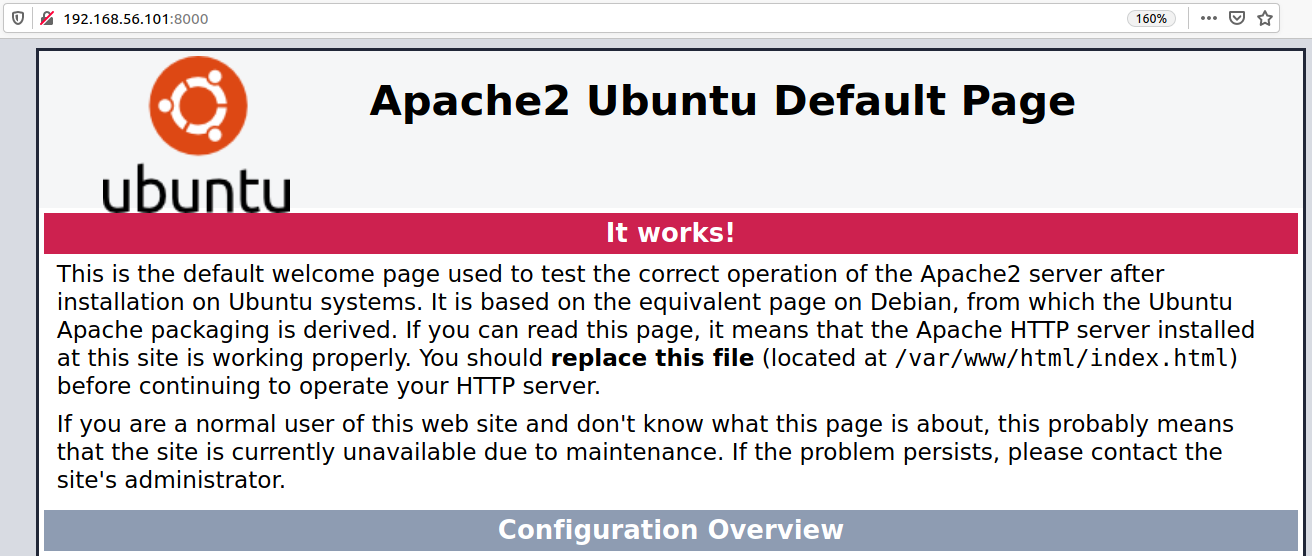
\includegraphics[width=140mm]{imgs/apache-page1}}
	\subfigure[M2, al puerto por efecto (80).]{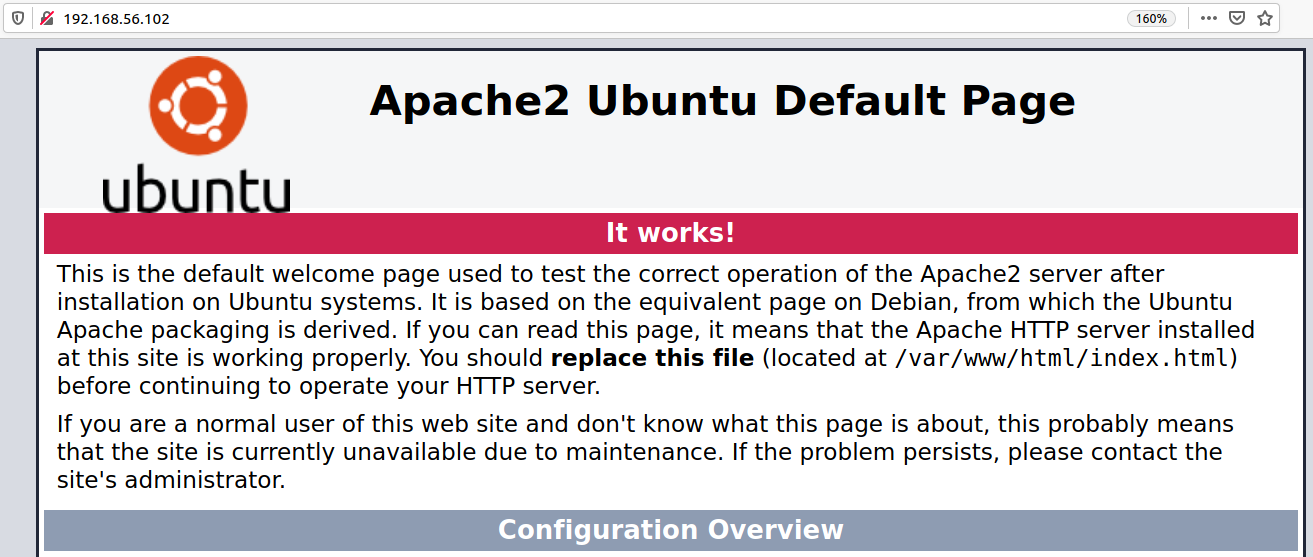
\includegraphics[width=140mm]{imgs/apache-page2}}
	\caption{El servicio Apache funciona correctamente, hemos cambiado el puerto de escucha en M1.}
	\label{fig:apache-page}
\end{figure}

Creamos el fichero \texttt{/var/www/html/ejemplo.html} en ambas máquinas. Mostramos el de la máquina 1.

\begin{Verbatim}[tabsize=4]
<html>
	<head>
		<meta charset="UTF-8">
	</head>
	<body>
		Web de dxabezas para SWAP (máquina 1) </br>
		Email: dxabezas@correo.ugr.es
	</body>
</html>	
\end{Verbatim}

Desde el anfitrión visualizamos el fichero correctamente en ambas máquinas:

\begin{figure}[H]
	\centering
	\subfigure[Ejemplo de la máquina 1.]{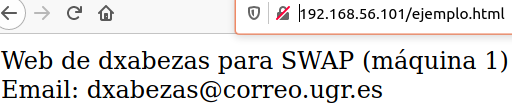
\includegraphics[width=120mm]{imgs/ejemplo-m1}}
	\subfigure[Ejemplo de la máquina 2.]{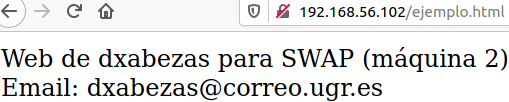
\includegraphics[width=120mm]{imgs/ejemplo-m2}}
	\caption{Archivos de ejemplo de ambas máquinas.}
	\label{fig:ejemplo}
\end{figure}

\subsubsection{Redirección de puertos}

En la máquina 1 atendemos peticiones desde el puerto 8000. Redireccionaremos las peticiones al puerto 80 para que se atiendan desde el
8000. Debemos hacer que Apache escuche en ambos puertos escribiendo \texttt{Listen 8000} y \texttt{Listen 80} en
 \texttt{/etc/apache2/ports.conf}.

A continuación seguimos las instrucciones de \\ \href{https://stackoverflow.com/questions/8541182/apache-redirect-to-another-port}
{https://stackoverflow.com/questions/8541182/apache-redirect-to-another-port}.

En \texttt{/etc/apache2/sites-enabled/000-default.conf}, añadimos el siguiente bloque:

\begin{Verbatim}[tabsize=4]
	<VirtualHost *:80>
		ProxyPreserveHost On
		ProxyRequests Off
		ProxyPass / http://localhost:8000/
		ProxyPassReverse / http://localhost:8000/
	</VirtualHost>
\end{Verbatim}

Ahora tenemos que añadir los módulos \texttt{proxy} y \texttt{proxy\_http}. Finalmente, reiniciamos el servicio.

\begin{verbatim}
	sudo a2enmod proxy
	sudo a2enmod proxy_http
	sudo systemctl restart apache2
\end{verbatim}

Ahora M1 es capaz de servir los archivos desde el puerto por defecto:

\begin{figure}[H]
	\centering
	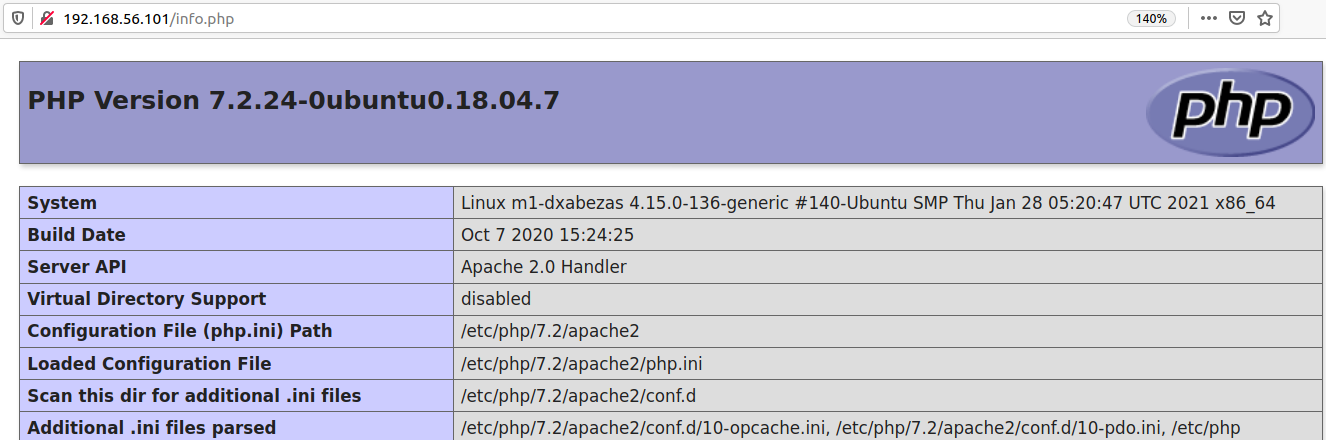
\includegraphics[width=160mm]{imgs/port-redirection}
	\caption{M1 sirve el fichero \texttt{/var/www/html/info.php} (que añadimos en la Sección \ref{sec:php}) ante una petición al puerto 80,
		 que redirige al 8000.}
	\label{fig:port-redirection}
\end{figure}

\subsubsection{Directorios virtuales}

Serviremos un directorio en \texttt{home} de la máquina 1. Creamos dos ficheros: \texttt{/home/dxabezas/carpeta/hola.html},
\texttt{/home/dxabezas/carpeta/hello.html}, con los mensajes ``Hola Mundo!'' y ``Hello World!''. A continuación, creamos un link simbólico
 de \texttt{carpeta} en \texttt{/var/www/html}

\begin{lstlisting}
	sudo ln -s ~/carpeta /var/www/html/carpeta
\end{lstlisting}

Ahora Apache puede servir ambos archivos:

\begin{figure}[H]
	\centering
	\subfigure[Directorio \texttt{carpeta}.]{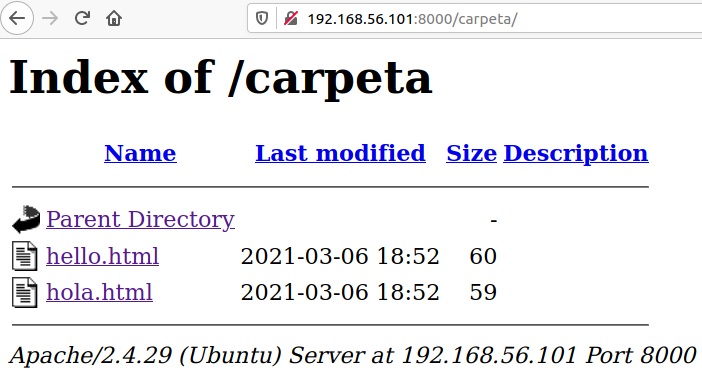
\includegraphics[width=100mm]{imgs/carpeta}}
	\subfigure[Archivo \texttt{/home/dxabezas/carpeta/hello.html}.]{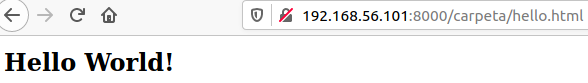
\includegraphics[width=140mm]{imgs/hello}}
	\caption{Gracias al enlace simbólico, Apache puede servir un subdirectorio de \texttt{home}.}
	\label{fig:virtual}
\end{figure}

\subsection{MySQL}

A continuación instalamos MySQL, tanto el servicio de servidor como de cliente

\begin{verbatim}
	sudo apt install mysql-client mysql-server
\end{verbatim}
Con \texttt{sudo systemctl status mysql.service}, comprobamos que el servicio está en marcha. Procedemos a la instalación
segura con \texttt{sudo mysql\_secure\_installation}. Nos hace varias preguntas para configurar la seguridad, en ambas máquinas:

\begin{itemize}
	\item No establecemos el plugin de validación de contraseñas, que obliga a que las contraseñas sean seguras.
	\item Elegimos \textbf{Swap1234} como contraseña para el usuario root de MySQL.
	\item Eliminamos el usuario anónimo para pruebas, compromete la seguridad de la base de datos una vez en producción.
	\item Deshabilitamos el remote root login, el root deberá loguearse desde localhost.
	\item Eliminamos la base de datos de test para la que todo el mundo tiene privilegios, compromete la seguridad en producción.
	También se eliminan los privilegios sobre esta BD en la tabla de privilegios.
	\item Recargamos la tabla de privilegios para hacer estos cambios efectivos.
\end{itemize}

Ya podemos acceder con \texttt{sudo mysql -u root -p=Swap1234}, o \texttt{-p} para que nos solicite la contraseña a continuación.

\begin{figure}[H]
	\centering
	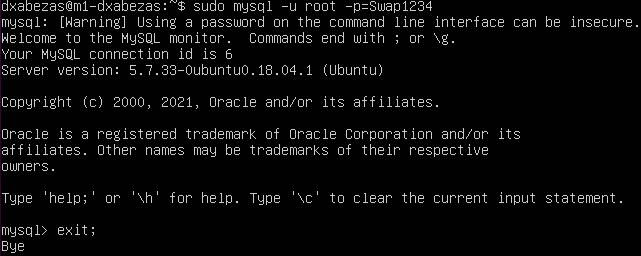
\includegraphics[width=160mm]{imgs/mysql}
	\caption{Acceso a MySQL en la máquina 1.}
	\label{fig:mysql}
\end{figure}

\subsection{PHP} \label{sec:php}

Instalamos PHP con \texttt{sudo apt install php}, automáticamente nos avisa de que va a instalar la versión 7.2 y de algunos paquetes
que necesita como \texttt{php7.2-json} y \texttt{libapache2-mod-php7.2}.

Para comprobar que funciona, creamos un fichero \texttt{/var/www/html/info.php} con el contenido

\begin{verbatim}
	<?php
	phpinfo();
	?>
\end{verbatim}

y comprobamos que se sirve correctamente desde la máquina anfitriona.

\begin{figure}[H]
	\centering
	\subfigure[Máquina 1, en la que cambiamos el puerto de HTML.]{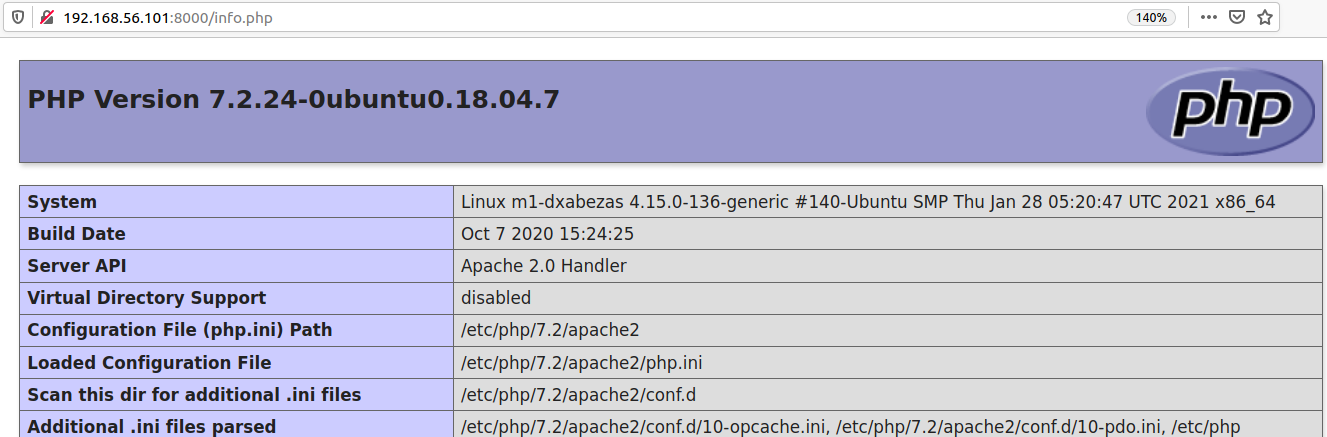
\includegraphics[width=160mm]{imgs/php1}}
	\subfigure[Máquina 2.]{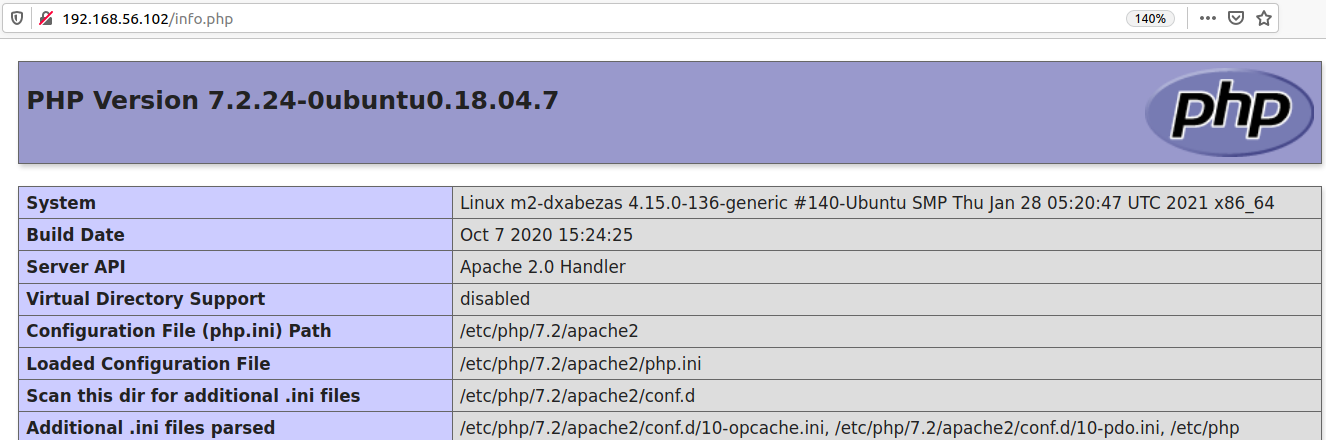
\includegraphics[width=160mm]{imgs/php2}}
	\caption{Desde la máquina anfitriona, comprobamos que PHP funciona correctamente en ambas máquinas.}
	\label{fig:php-info}
\end{figure}

\section{cURL}

Instalamos cURL:

\begin{verbatim}
sudo apt install curl
\end{verbatim}
nos dice en ambas máquinas que ya está instalado y en su última versión.

Como primera prueba, obtenemos fichero \texttt{/var/www/html/ejemplo.html} de la máquina 1 desde la 2:

\begin{figure}[H]
	\centering
	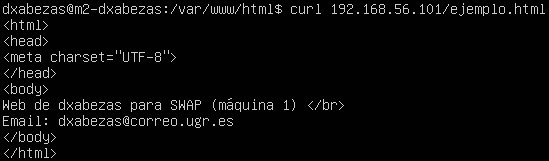
\includegraphics[width=120mm]{imgs/curl}
	\caption{Visualizamos el ejemplo de M1 en M2 mediante cURL.}
	\label{fig:curl}
\end{figure}

Con la opción \texttt{-o}, podemos descargar el fichero en la máquina 2:

\begin{figure}[H]
	\centering
	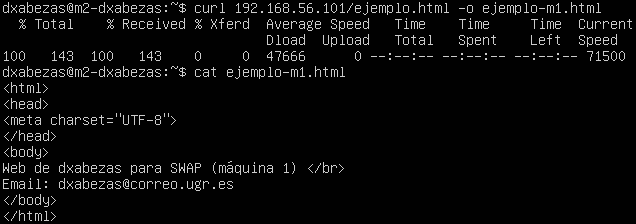
\includegraphics[width=140mm]{imgs/curl-o}
	\caption{Descargamos el ejemplo de M1 en M2 mediante cURL.}
	\label{fig:curl-o}
\end{figure}

La opción \texttt{-O} es similar, guarda el fichero con el mismo nombre con el que está subido. Esta vez hacemos la petición
al puerto 8000 en lugar de al puerto por defecto (80).

\begin{figure}[H]
	\centering
	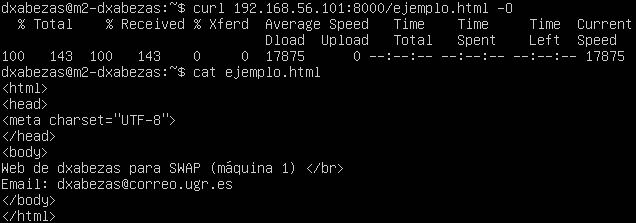
\includegraphics[width=140mm]{imgs/curl-O}
	\caption{Descargamos el ejemplo de M1 en M2 mediante cURL.}
	\label{fig:curl-O}
\end{figure}

Todas las peticiones que hemos hecho son GET (por defecto). Si quisiésemos realizar otra petición (como POST,
PUT, COPY o DELETE), tendríamos que explicitarla con la opción \texttt{--request <peticion>}.

Por ejemplo, podríamos subir un JSON con el siguiente comando:

\begin{verbatim}
	curl --location --request POST '<direccion>' --header 'Content-Type: application/json'
	--data-raw '{nombre: "David", apellidos: "Cabezas Berrido"}'
\end{verbatim}

\subsection{Cookies}

Para utilizar cookies con cURL, debemos conocer dos opciones. La primera es \texttt{-c} o \texttt{--cookie-jar}, con la que se indica
el nombre de un archivo para almacenar las cookies. Por ejemplo:

\begin{verbatim}
	curl -c cookie.txt https://www.google.com
\end{verbatim}

Se crea el archivo \texttt{cookie.txt}:

\begin{figure}[H]
	\centering
	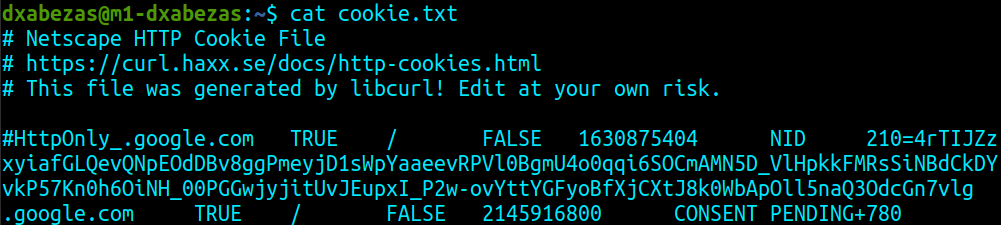
\includegraphics[width=130mm]{imgs/cookie-c}
	\caption{Se ha creado el archivo con la cookie.}
	\label{fig:cookie-c}
\end{figure}

La segunda opción es \texttt{-b} o \texttt{--cookie}, para enviar cookies. Por ejemplo:

\begin{verbatim}
curl -b cookie.txt https://www.google.com
\end{verbatim}

\end{document}